\section{Implementation}
The main package for this application is \texttt{eu.sportperformancemanagement}. Every part of the architecture is defined in its own package. Since the client is purely web-based, it is not part of a Java package. There is also a \texttt{common} package, which contains code that is shared over multiple parts. This section includes some UML diagrams, but they are not always complete (e.g. getters and setters are not there). This would result in much superfluous information which is not necessary to understand the application from a technical point of view.

\subsection{eu.sportperformancemanagement.common}
The most important classes of the common package are shown in the UML diagram of figure \ref{fig:uml_common}. \texttt{LocationPacket} and \texttt{LocationRequest} objects are only used to communicate within the system, so they provide an easy way to marshall their information with almost no overhead. \texttt{Match} and \texttt{Player} classes both have a class which can make and parse JSON of (arrays of) these objects. 

\begin{figure}
\centering
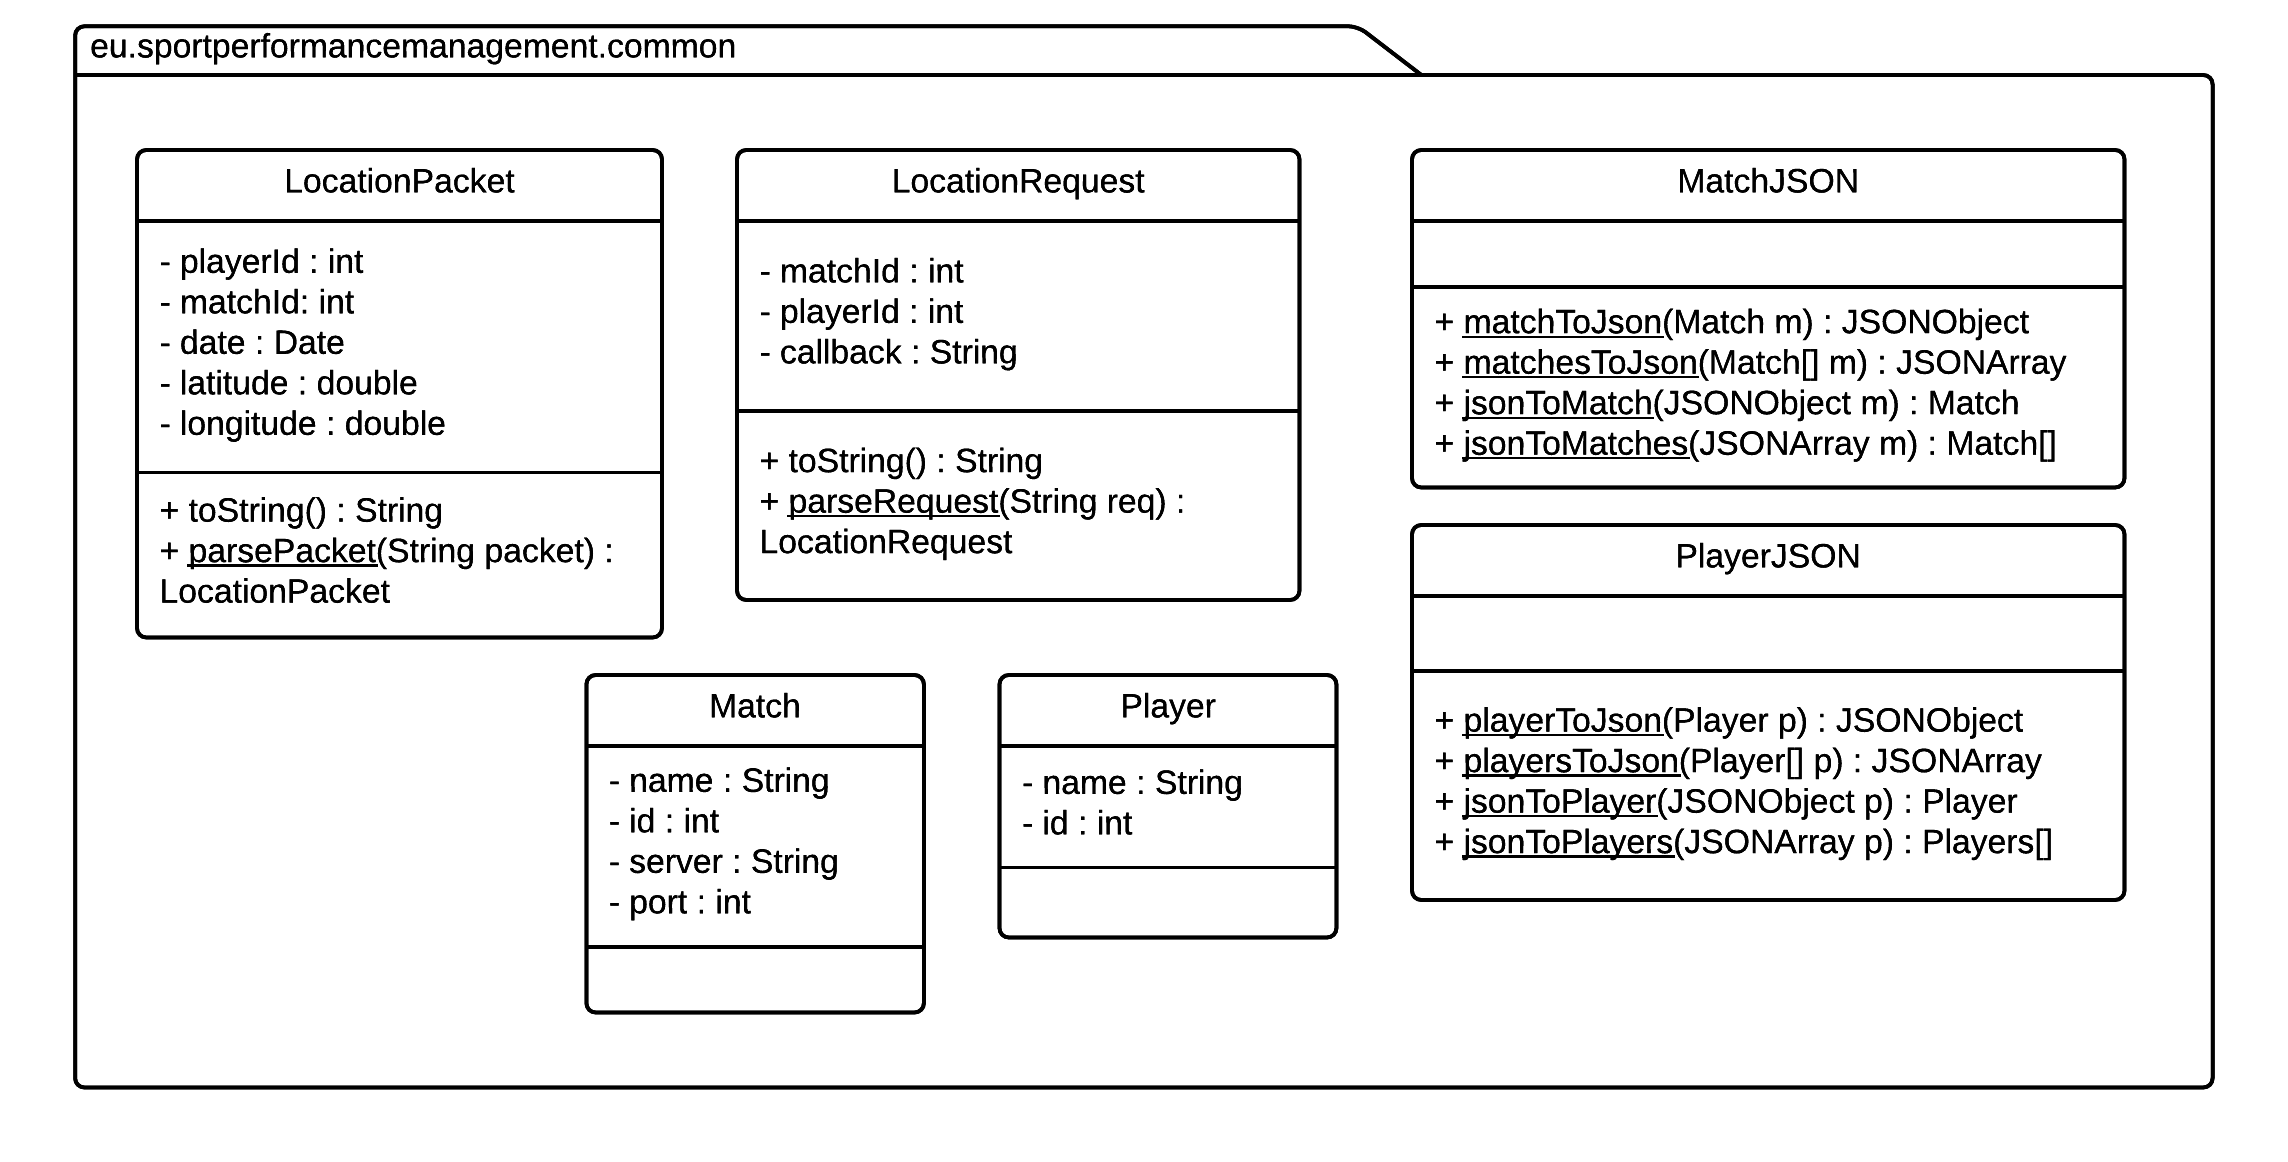
\includegraphics[width=\textwidth]{img/uml_common.png}
\caption{The UML diagram for the common package.}
\label{fig:uml_common}
\end{figure}

\subsection{eu.sportperformancemanagement.player}
As said in the Architecture section, the sports(wo)men are modelled using an Android app. There are three activities (i.e. "pages"): showing a list of matches, setting the player and the match detail activity. The last activity is used to start monitoring locations for a certain match. The match detail activity uses two classes to monitor locations and send location updates to the DataServers. \texttt{LocationMonitor} listens for locations, using the Google API client provided in the Android framework, and sends the location to \texttt{LocationSender}, which makes a \texttt{LocationPacket} and sends it over UDP to the DataServer connected to this match (figure \ref{fig:dataflow}).

\subsection{eu.sportperformancemanagement.dataserver}
The DataServer has two important classes. First of all, \texttt{LocationListener} listens for incoming \texttt{LocationPackets} on a UDP socket and uses \texttt{LocationDAO} to store them in their local database. \texttt{QueueListener} listens on a Rabbit MQ channel for incoming \texttt{LocationRequest}s, indicated by a specific routing key as defined in \texttt{SpmConstants} in the common package. When this request comes in, it will use \texttt{LocationDAO} to fetch all locations for the given player and match and send them using a http POST request to the callback. 

\subsection{eu.sportperformancemanagement.webservice}
The Webservice is mainly a Jersey REST webservice. There are three resources available. \texttt{MatchesResource} and \texttt{PlayersResource} both provide a GET and POST endpoint on respectively \texttt{/matches} and \texttt{/players} where the user can get a list of all matches/players and create a new match/player. To handle communication with the database, a \texttt{MatchDAO} and \texttt{PlayerDAO} class is used. The third resource is \texttt{LocationResource}. When a GET request is made to \texttt{/locations/<match\_id>/<player\_id>}, a \texttt{LocationRequest} is created with the given match and player id. A unique callback is also generated and added to the request. This \texttt{LocationRequest} is sent to a RabbitMQ fanout exchange using \texttt{RequestEmitter}. The DataServers who receive this request make a http POST to the callback with all locations they have for this match and player.

\subsection{Client}
The client consists of a set of webpages. The first webpage shows a form where the coach can select a match and a player. Then a request is sent to the Webservice. On return, the webpages makes a heatmap using the Google Maps Api: \url{https://developers.google.com/maps/documentation/javascript/examples/layer-heatmap}. Furthermore, there are two pages where the coach can create new players and matches using POST requests to the webservice.


\subsection{Communication}
All communication between components is depicted in a data flow diagram in figure \ref{fig:dataflow}.
\begin{description}
\item[Player - DataServer] \hfill \\
The player sends their location data to the DataServer over UDP sockets. Since a lot of locations can be sent, we choose for the faster UDP protocol. The data that is sent is a \texttt{LocationPacket} object from the common package. The \texttt{toString()} result is send, and this is parsed at the DataServer using \texttt{parsePacket}.

\item[Player - Webservice] \hfill \\
Player uses the REST service defined at the Webservice to load the list of matches and players. For this, the REST endpoints \texttt{/matches} and \texttt{/locations} can be accessed with a GET request and can return the following results
\begin{itemize}
    \item \emph{200 - OK} with a JSON array of matches / players, made by \texttt{MatchJSON} (or Player).
    \item \emph{500 - Internal Server Error} when loading the resources from the database failed.
\end{itemize}

\item[Client - Webservice] \hfill \\ 
The client uses the same REST endpoints as defined in Player - Webservice for loading lists of players and matches. In addition, it uses the endpoints for creating new matches and players. These can be accessed by making a POST request to the same endpoints. For creating a match, the \texttt{name, server} and \texttt{port} field need to be provided. For players, only \texttt{name} is necessary. Both endpoints can return the following:
\begin{itemize}
    \item \emph{201 - Created} with a JSON representation of the created object.
    \item \emph{409 - Conflict} when a resource with the given \texttt{name} already exists.
    \item \emph{500 - Internal Server Error} when inserting the resources in the database failed.
\end{itemize}
In addition, the Client can request locations of a certain \texttt{matchId} and \texttt{playerId} at \\ \texttt{/locations/{matchId}/{playerId}}. This can return the following:
\begin{itemize}
    \item \emph{200 - OK} with a JSON array of locations.
    \item \emph{500 - Internal Server Error} when the locations could not be loaded.
\end{itemize}


\item[Webservice - DataServer] \hfill \\
When the Webservice receives a request for locations of a certain match and player, it will ask all DataServers if they can provide the locations they know. This is done using RabbitMQ. The Webservice sends a \texttt{LocationRequest} to the exchange, which uses a fanout with specific routing key to send the request to all DataServers, which are listening on the queue. When the DataServer receives a message with the specific routing key, they parse the \texttt{LocationRequest}, fetch the locations from the database and POST's them to the callback. The Webservice waits a predefined number of milliseconds before returning all locations it received on the POST callback.


\begin{figure}[h]
\centering
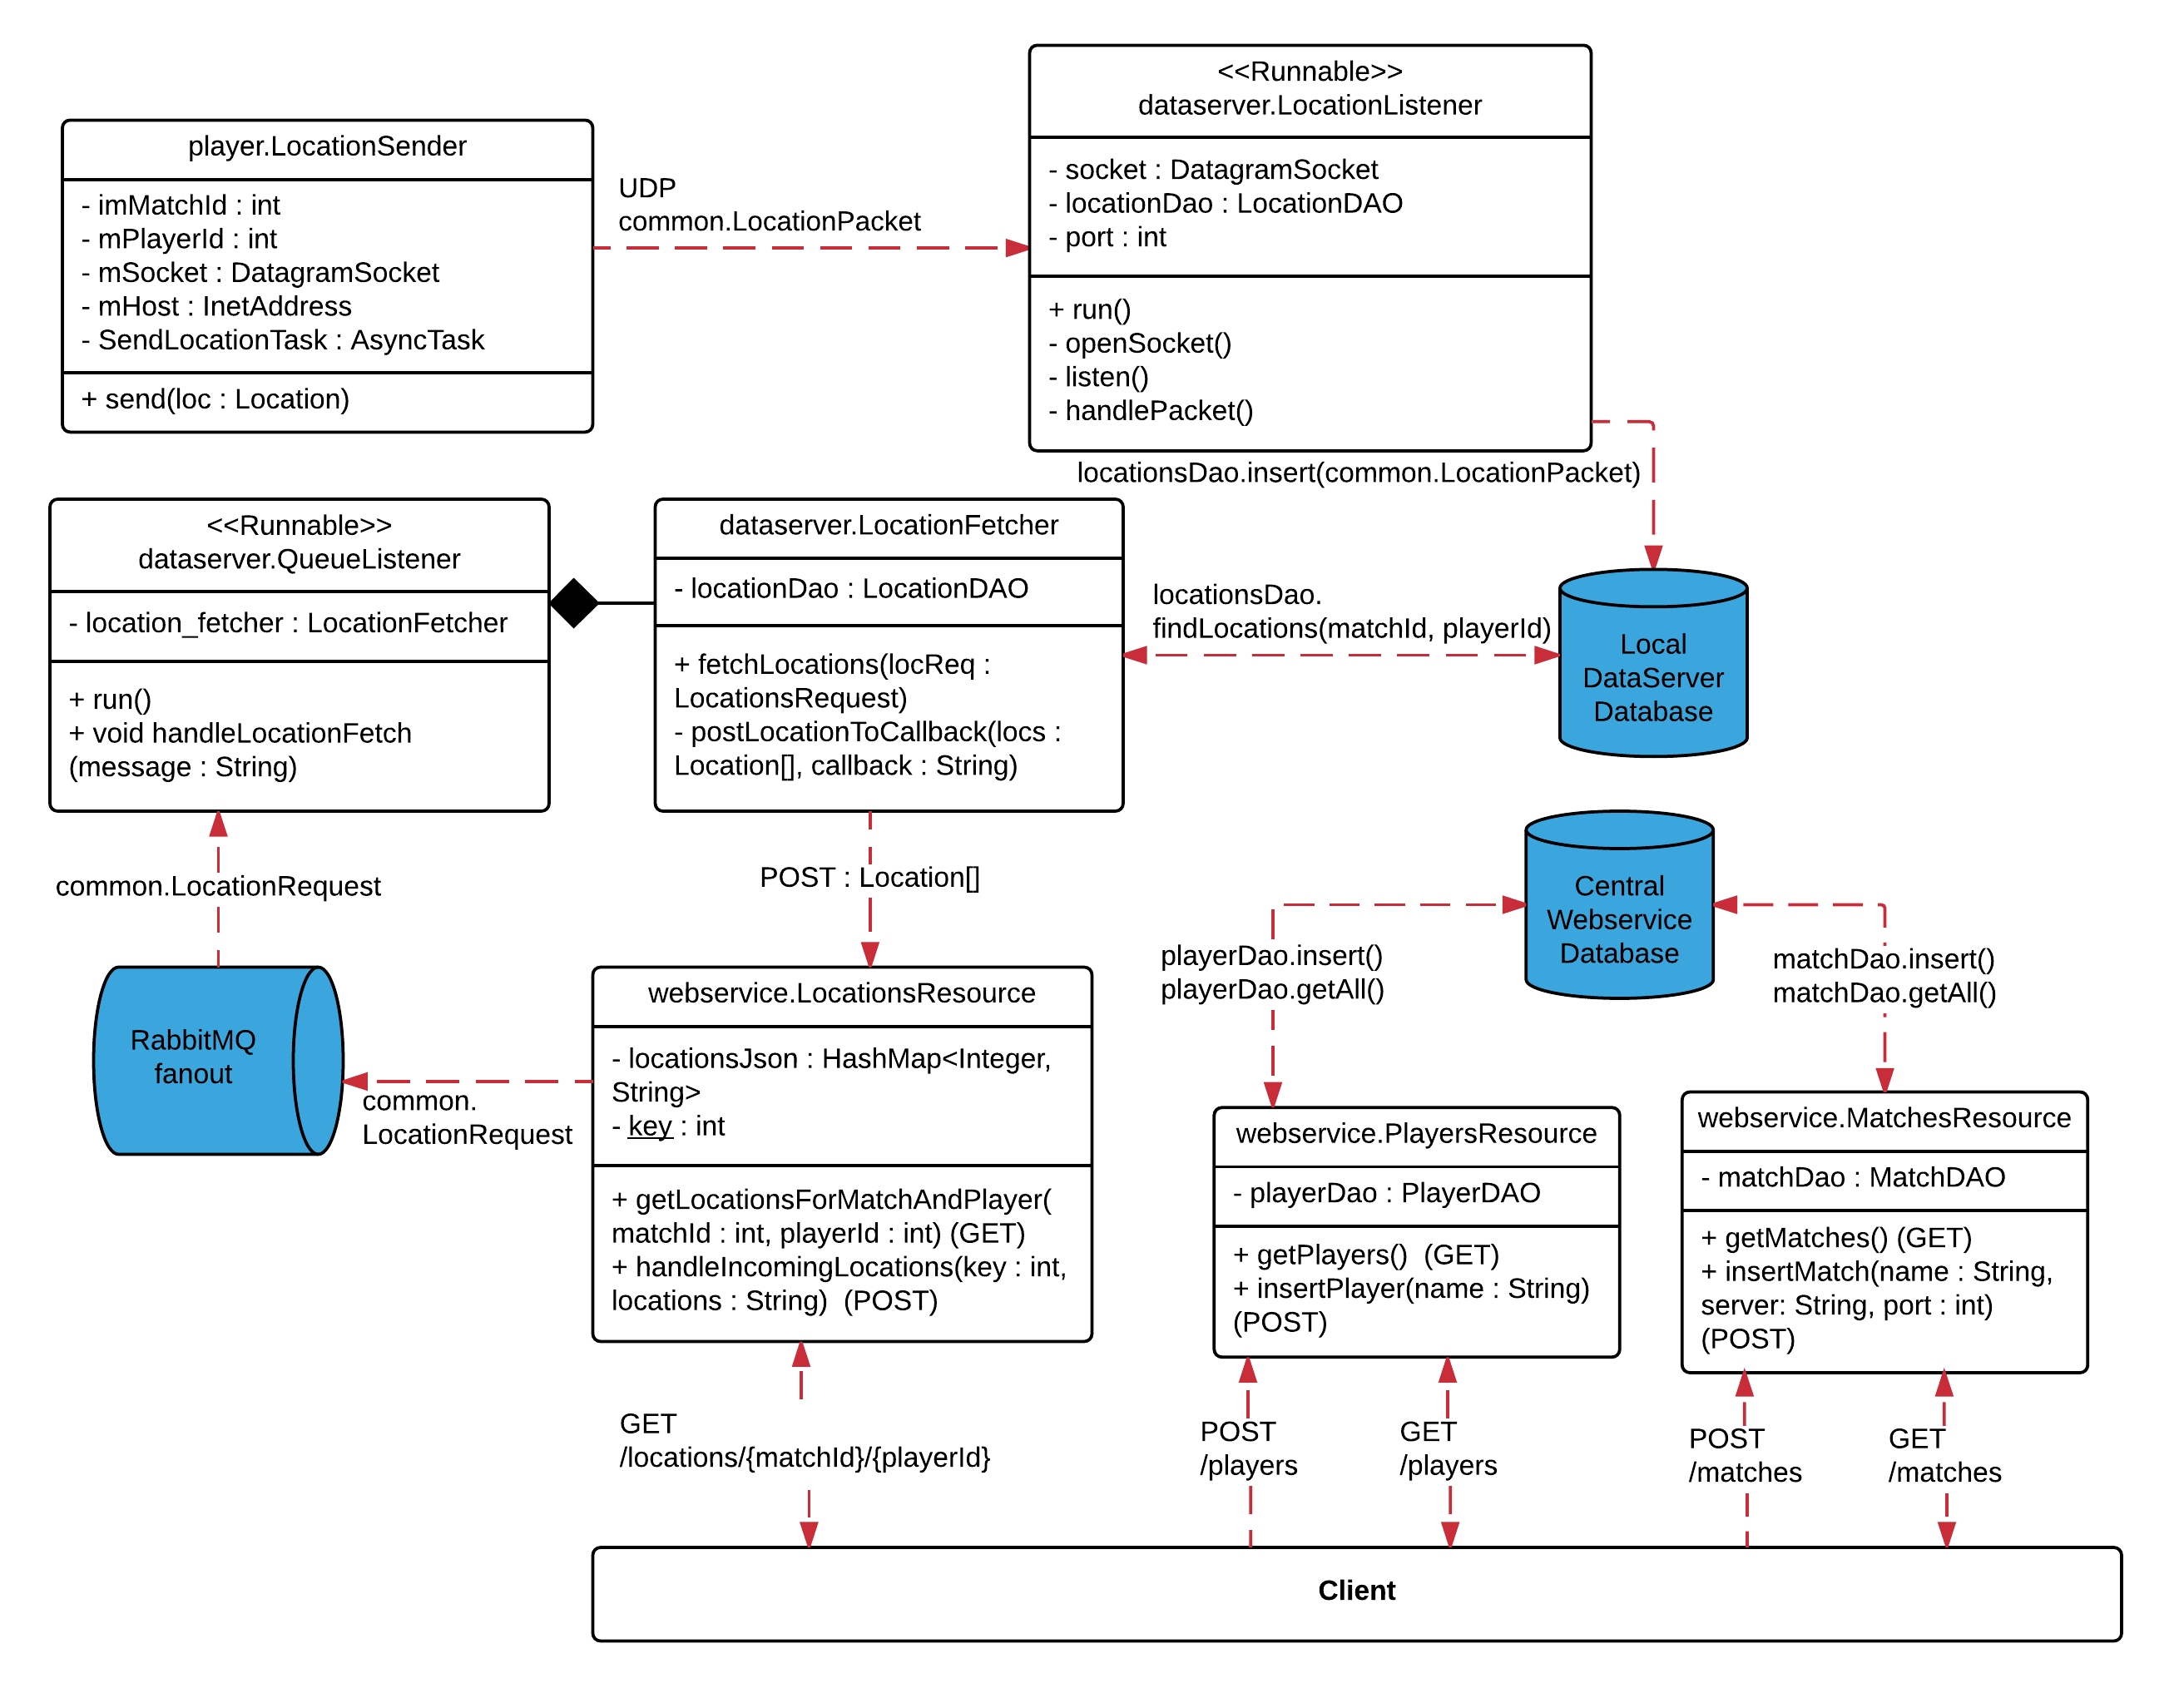
\includegraphics[width=0.9\textwidth]{img/dataflow.png}
\caption{The data flow between different elements of the application. Note that the Player also communicates with the webserver to get players and matches.}
\label{fig:dataflow}
\end{figure}

\end{description}